\section{eo\-Bool\-Flip Class Reference}
\label{classeo_bool_flip}\index{eoBoolFlip@{eoBoolFlip}}
a simple boolean mutation - to be used in generic eo\-Op's  


{\tt \#include $<$eo\-Bool\-Flip.h$>$}

Inheritance diagram for eo\-Bool\-Flip::\begin{figure}[H]
\begin{center}
\leavevmode
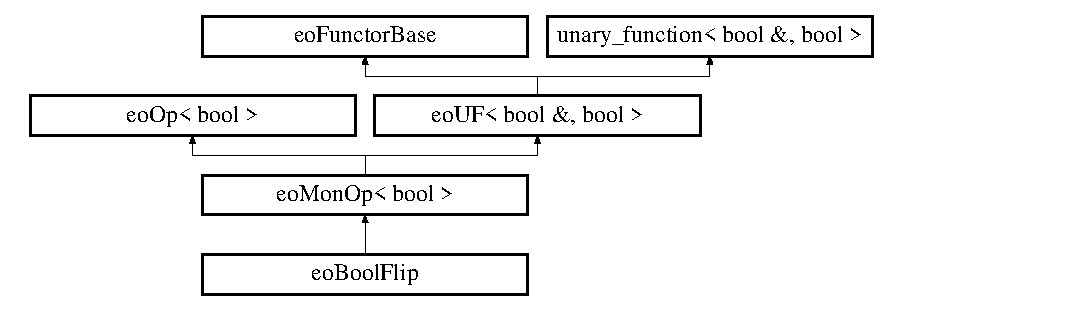
\includegraphics[height=3.73333cm]{classeo_bool_flip}
\end{center}
\end{figure}
\subsection*{Public Member Functions}
\begin{CompactItemize}
\item 
bool {\bf operator()} (bool \&\_\-b)\label{classeo_bool_flip_a0}

\begin{CompactList}\small\item\em simply flips the boolean argument \item\end{CompactList}\item 
virtual string {\bf class\-Name} () const \label{classeo_bool_flip_a1}

\begin{CompactList}\small\item\em inherited {\bf class\-Name()}{\rm (p.\,\pageref{classeo_bool_flip_a1})} \item\end{CompactList}\end{CompactItemize}


\subsection{Detailed Description}
a simple boolean mutation - to be used in generic eo\-Op's 



Definition at line 32 of file eo\-Bool\-Flip.h.

The documentation for this class was generated from the following file:\begin{CompactItemize}
\item 
eo\-Bool\-Flip.h\end{CompactItemize}
